\section{Analysis}
\label{sec:analysis}

\subsection{Model Performance}

In our experiments, we ran four models in sequence to find a trend in performance. This section presents a discussion and evaluation of the four models: Base Model, LDP Model, PolyP Model, and Hybrid Model across three of  DIALECTBENCH's \cite{Faisal:24} tasks: Natural Language Inference (NLI), Machine Reading Comprehension (MRC), and Machine Translation (MT). 

\subsubsection{Natural Language Inference (NLI)}

The results in Table~\ref{tab:model-performance} show that the \textbf{Base Model} achieves the highest NLI F1 score (\(0.645 \pm 0.106\)), suggesting a stronger generalization in inferring logical relationships in cross-lingual dialogue. Compared to the Base Model, the inclusion of linguistic diversity in the \textbf{LDP Model} results (0.617 $\pm $ 0.085) in a performance drop of approximately \(4.34\%\), indicating potential noise introduced by the inclusion of a high-resource language and contextual markers in the prompts.

The \textbf{PolyP Model} (\(0.595 \pm 0.093\)) demonstrates a further performance decline of approximately \(7.75\%\) relative to the Base Model, likely due to increased complexity in balancing multilingual exemplars and dialectal features. The \textbf{Hybrid Model} (\(0.561 \pm 0.081\)) experiences the largest drop of approximately \(13.02\%\) compared to the Base Model, suggesting that combining techniques may lead to overcompensation to specific dialectal and contextual features.


\subsubsection{Machine Reading Comprehension (MRC)}

The results in Table~\ref{tab:model-performance} show that the \textbf{Hybrid Model} achieves the highest MRC F1 score (\(0.924 \pm 0.042\)), demonstrating that a combined approach of Linguistically Diverse Prompting (LDP) and Polyglot Prompting (PolyP) enhances the model's understanding of nuanced textual information in a cross-lingual context. The \textbf{PolyP Model} (\(0.903 \pm 0.056\)) also performs well, leveraging multilingual exemplars for improved comprehension.

The \textbf{Base Model} (\(0.803 \pm 0.065\)) performs reasonably well but lacks the contextual depth provided by cultural and conversational markers. Interestingly the \textbf{LDP Model} (\(0.755 \pm 0.098\)) under-performs relative to the Base Model. This suggests that combining contextual markers (\(c_j\)) with multilingual exemplars significantly improves comprehension tasks in most scenarios, and that utilizing a high resource language (SAE) in this particular case doesn't improve the model's comprehension in a cross-lingual setting. With an increase in score by more than $10\%$ the \textbf{PolyP Model} and \textbf{Hybrid Model} results suggest that polyglot prompting might significantly improve the model's comprehension with our low resource language (Haitian Creole) with further contextual enhancement found in the \textbf{Hybrid Model}'s prompting style also improving performance. 

\subsubsection{Machine Translation (MT)}

Table~\ref{tab:mt-bleu-performance} shows that the \textbf{Hybrid Model} achieves the highest BLEU score (\(18.057 \pm 10.703\)) followed by the \textbf{PolyP Model} (\(6.507 \pm 8.866\)). Though these scores are all far below average, the \textbf{Hybrid Model} performs roughly 2.775 times better than it's runner-up. This suggests that the inclusion of $D_1$ (Main Dialect/Language), $D_2$ (High Resource Language), and a $D_3$ (Polyglottal Language) with contextual markers might significantly improve a model's cross-lingual translational ability.

The \textbf{LDP Model} (\(3.804 \pm 4.009\)) shows minimal improvement over the \textbf{Base Model} (\(2.456 \pm 3.359\)), indicating that linguistic diversity positively impacts translation tasks. However, the results suggest that the combination of LDP and PolyP techniques, as employed in the Hybrid Model, is crucial for achieving higher-quality translations in low-resource languages.

\subsubsection{Trends}

Across all tasks, a clear trade-off emerges between model complexity and task-specific performance. The \textbf{Base Model} excels in NLI tasks, where logical consistency and simplicity are critical. In contrast, the \textbf{Hybrid Model} consistently outperforms others in MRC and MT tasks, demonstrating the effectiveness of integrating cultural and contextual markers (\(c_j\)) with multilingual exemplars (\(z_i, e_{z_i}\)). This is highlighted in Figure 5 where the trade-off is presented in a steep slope seen in the third evaluation run.

The decline in NLI performance for LDP and PolyP models highlights the difficulty of balancing linguistic diversity with logical inference. In contrast, the gains in MRC and MT tasks underscore the importance of cultural and conversational adaptation, which enhances the model's understanding and generation capabilities across dialects and languages.

\subsection{Error Analysis}
Our evaluation of the Base, LDP, PolyP (Polyglot Prompting), and Hybrid (LDP + Polyglot) models highlights distinct patterns in errors, closely aligned with the performance trends discussed earlier. These patterns reflect the interplay between linguistic diversity, dialect-specific adaptability, and cultural nuances across tasks. Below, we provide a detailed breakdown of error types observed across models.

\subsubsection{Task-Specific Performance}
While the \textbf{Base Model} excelled in Natural Language Inference (NLI), its performance dropped significantly in Machine Reading Comprehension (MRC) and Machine Translation (MT). This suggests that simple prompting style with minimal contextual inclusion are beneficial for logical reasoning tasks but insufficient for tasks requiring deeper cross-lingual understanding and nuanced cultural adaptation. Conversely, the \textbf{Hyrbid Model} showed superior performance in MRC and MT but suffered a substantial decline in NLI, demonstrating that increased complexity can introduce trade-offs in logical reasoning due to increased noise.

We also noted that inclusion of dialectal and multilingual features in tags, as seen in the \textbf{LDP Model}, introduced noise that negatively impacted performance and possibly standard deviations as seen in Figure~\ref{fig:nli-analysis}, particularly in tasks requiring logical consistency. The \textbf{PolyP Model}, while better equipped to handle multilingual exemplars, struggled with overlapping dialect markers and cultural expressions, highlighting the difficulty of balancing linguistic diversity with task-specific requirements. The \textbf{ Model}, despite its improvements, exhibited errors stemming from the overcompensation for dialectal and contextual markers, particularly in ambiguous scenarios.

These findings emphasize the need for improvements in both the model and the evaluation framework. Expanding training datasets to include more diverse and complex examples, particularly from low-resource dialects, could mitigate these issues. Furthermore, refining evaluation metrics to better accommodate unconventional but valid outputs would enable a more comprehensive assessment of model performance. Addressing these gaps would enhance model robustness and adaptability across diverse linguistic contexts.

\paragraph{Ambiguity in Linguistic Tags:}
Distinguishing nuanced linguistic features, such as overlapping markers for AAVE and Haitian Creole, posed significant challenges. The use of BGE rather than an LLM for led to ambiguous tagging. This caused misclassification or blending of linguistic features as an overcompensation. While the \textbf{LDP Model} improved in capturing dialect-specific tags, inconsistencies arose in more complex scenarios. The \textbf{Hybrid Model} handled ambiguous tags more effectively but struggled during rapid transitions between linguistic contexts. This would explain why the more complex model's struggled in logic based tasks (NLI) given in the prompts.

\begin{figure}[h!]
    \centering
    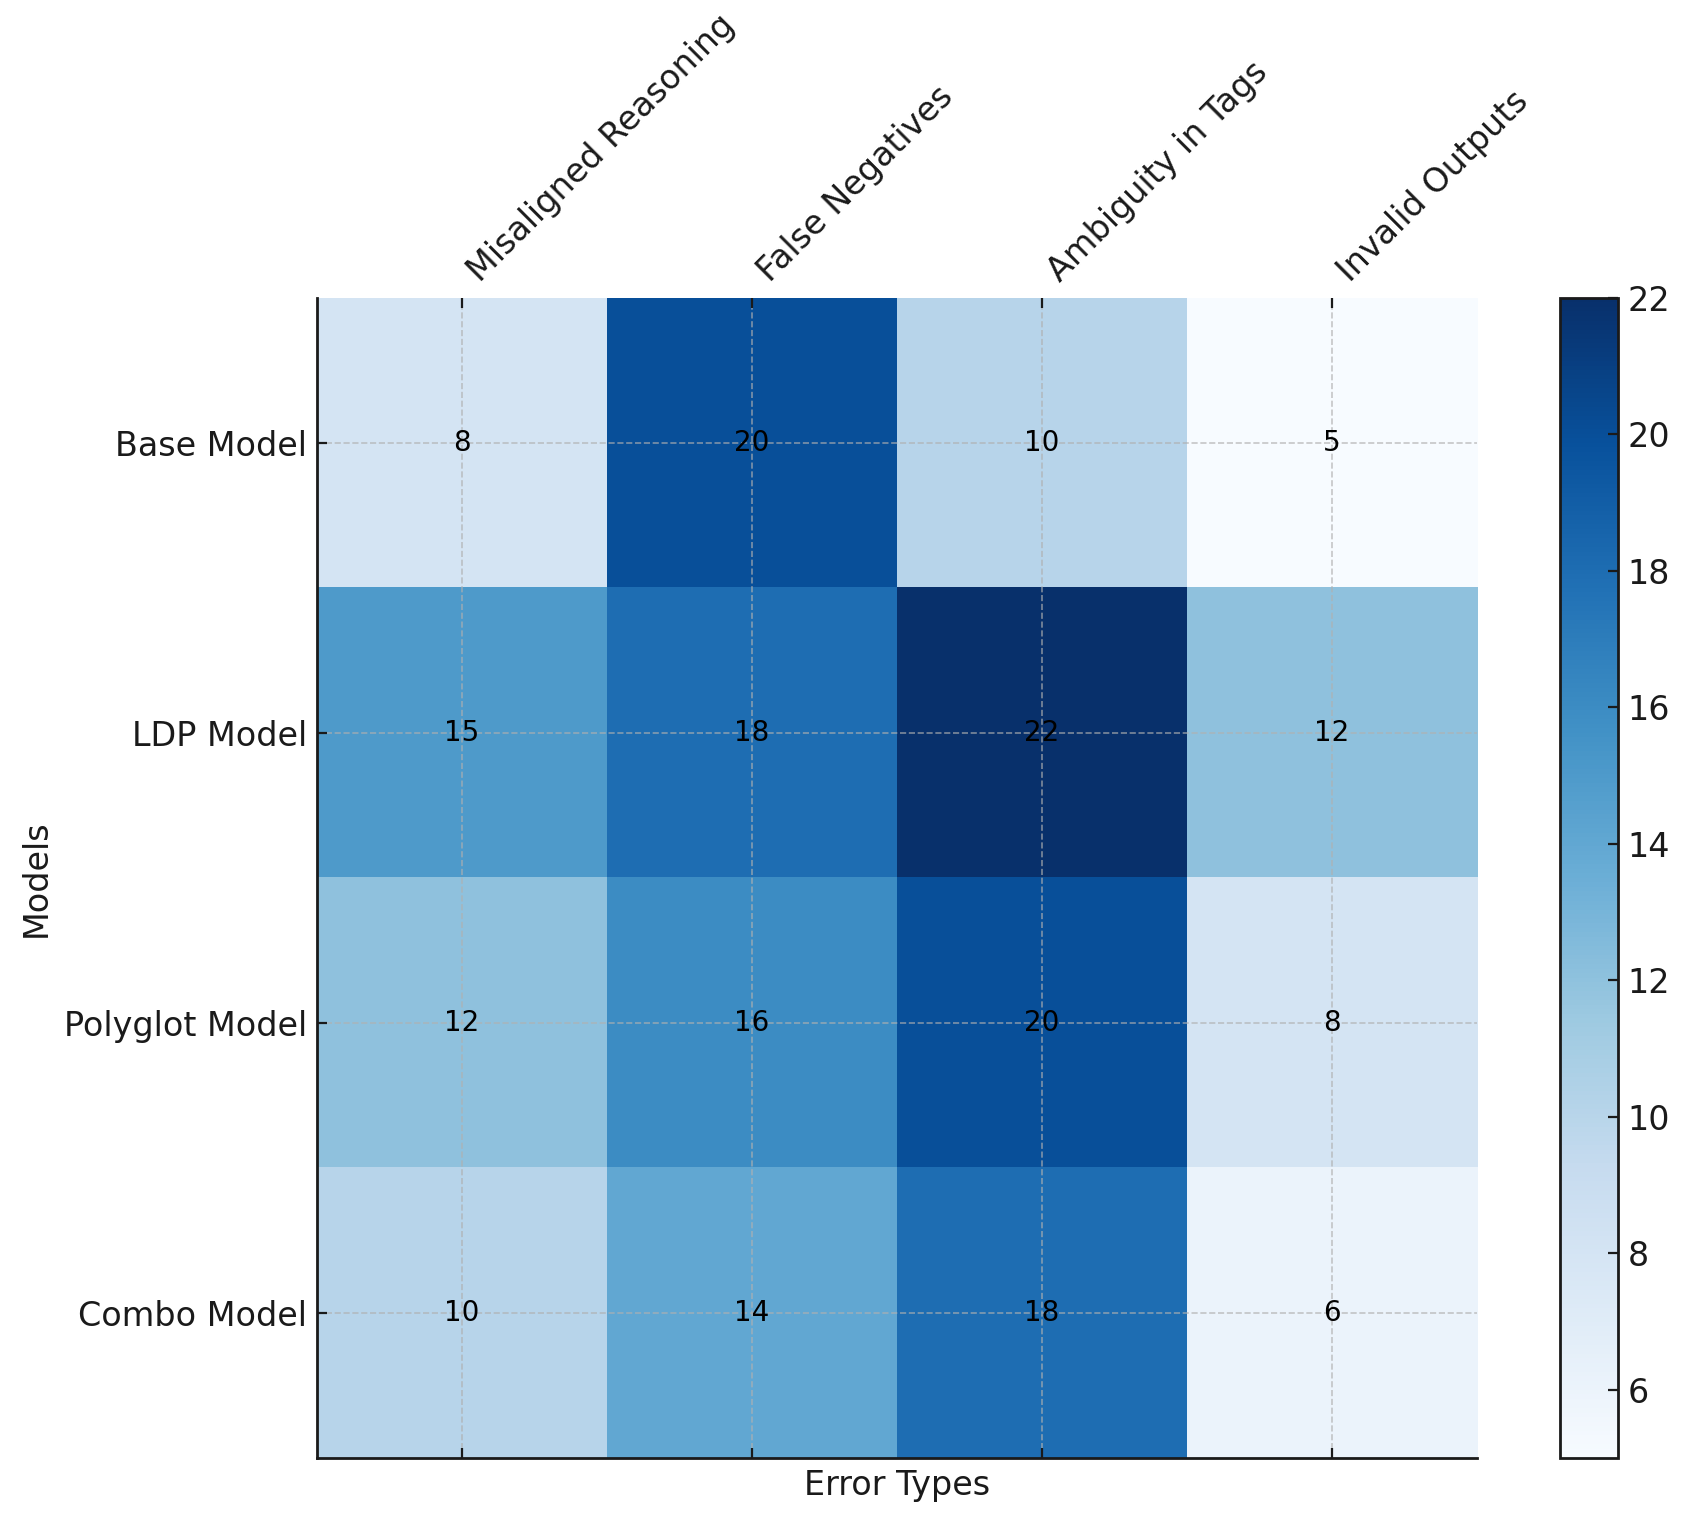
\includegraphics[width= \linewidth]{output.png}
    \caption{NLI Task Confusion Matrix}
    \label{fig:enter-label}
\end{figure}

\paragraph{Errors in Evaluation Metrics:}
During evaluation, certain entries produced blank or invalid values for metrics such as NLI F1, MT BLEU, or MRC F1. These errors often stemmed from the model's inability to distinguish tags for prompts with ambiguous phrasing, low-resource dialectal expressions, or complex linguistic structures. Additionally, evaluation metrics reliant on lexical overlap or strict logical alignment failed to capture meaningful outputs when models deviated significantly from expected formats.

\subsubsection{Table of Errors and Outputs}
Table~\ref{tab:error-analysis} provides examples of errors observed across models. Each row includes an input prompt, the generated output, the expected output, and the specific type of error identified. These examples illustrate the challenges in maintaining linguistic precision, cultural context, and idiomatic meaning.


\subsection{Discussion}
The results underscore the importance of task-specific adaptations in low-resource language processing. While NLI tasks benefit from simpler, generalizable models, MRC and MT tasks require more nuanced approaches that incorporate cultural, poly-glottal data, and conversational context. However, there are some key limitations we identified. 



\subsubsection{Limitations in Dataset Diversity}
A significant limitation lies in the diversity and coverage of the training datasets. Low-resource dialects, such as Haitian Creole and African American Vernacular English (AAVE), are underrepresented, leading to challenges in accurately capturing dialect-specific features. The lack of sufficient examples for dialect mixing and code-switching further exacerbates this issue, as evidenced by frequent misclassification and blending of linguistic features in the models' outputs.

\subsubsection{Limitations in Evaluation Metrics}
The reliance on standard evaluation metrics, such as F1 for NLI and MRC or BLEU for MT, introduces additional limitations. These metrics often fail to account for unconventional but valid outputs, particularly in low-resource language contexts. For instance, the BLEU scores for the MT task were notably low across all models with extreme standard deviations Figure~\ref{fig:mt-analysis}, even for the \textbf{Hybrid Model}, which achieved the highest score. This raises questions about whether BLEU effectively captures the quality of translations in cross-lingual and culturally nuanced scenarios, and if our BLEU scores are a proper indication of translation readability on a basic level. Similarly, blank or invalid metric values highlight the need for evaluation frameworks that can handle ambiguous phrasing and complex linguistic structures more effectively. Perhaps a model fine-tuned on the utilized low-resource language might yield significantly better translation scores while maintaining a similar trend of performance improvement across our four model structures.


\subsubsection{Future Direction}
We believe future work should focus on fine-tuning our model on multiple low-resource languages, as this might further improve translational and comprehension tasks in our combined model. Fine-tuning our model on Natural Language Inference Tasks would also prove to be useful in further studies, as we can then eliminate the disparity found in more complex models when carrying out logical tasks. 
Further testing should be done in other languages and there dialectal variations or similar tongues. For example, Basque and Spanish are both Latin-based languages but not dialects of each other. By including a dialect such Andalusian Spanish, we might be able to yield more results indicating that the \textbf{Hybrid Model} works in a broader cross-lingual context. 
Additionally, we aim to explore speech-to-speech transformations, allowing models to seamlessly process spoken inputs and generate accurate spoken outputs with nuanced responses that honor cultural and contextual cues.









